% Este trabalho está licenciado sob a Licença Atribuição-CompartilhaIgual 4.0 Internacional Creative Commons. Para visualizar uma cópia desta licença, visite http://creativecommons.org/licenses/by-sa/4.0/deed.pt_BR ou mande uma carta para Creative Commons, PO Box 1866, Mountain View, CA 94042, USA.

\chapter{Programação Estruturada}\label{cap_progest}
\thispagestyle{fancy}

\hl{No paradigma de programação estruturada, o programa é organizado em blocos de códigos}. Cada bloco tem uma entrada de dados, um processamento (execução de uma tarefa) e produz uma saída.

\begin{figure}[H]
  \centering
  \includegraphics[width=0.4\textwidth]{./cap_progest/dados/fig_fg_bloco/fig}
  \caption{Bloco de processamento.}
  \label{cap_progest:fig:fg_bloco}
\end{figure}

Blocos podem ser colocados em sequência, selecionados com base em condições lógicas, iterados ou colocados dentro de outros blocos (sub-blocos).

\section{Estruturas de um Programa}\label{cap_progest_sec_est}

\hl{Para escrever qualquer programa, apenas três estruturas são necessárias: \emph{sequência}, \emph{seleção/ramificação} e \emph{iteração}}.

\begin{figure}[H]
  \centering
  \includegraphics[width=0.4\textwidth]{./cap_progest/dados/fig_fg_bloco/fig}
  \caption{Bloco de processamento.}
  \label{cap_progest:fig:fg_bloco}
\end{figure}


\subsection{Sequência}

A estrutura de \hl{\emph{sequência}} apenas significa que \hl{os blocos de programação são executados em sequência}. Ou seja, a execução de um bloco começa somente após a finalização do bloco anterior.

\begin{figure}[H]
  \centering
  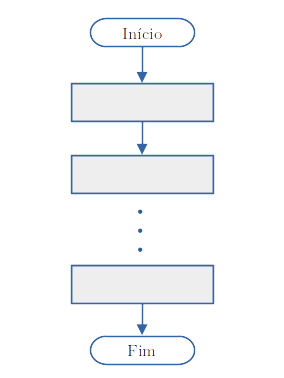
\includegraphics[width=0.4\textwidth]{./cap_progest/dados/fig_fg_sequencia/fig}
  \caption{Estrutura de sequência de blocos.}
  \label{cap_progest:fig:fg_sequencia}
\end{figure}

\begin{ex}
  O seguinte código computada a área do triângulo de base e altura informadas pela(o) usuária(o).
\begin{lstlisting}
#início

# bloco: entrada de dados
base = float(input('Digite a base:\n'))
altura = float(input('Digite a altura\n'))

# bloco: computação da área
area = base*altura/2

# bloco: saída de dados
print(f'Área = {area}')

#fim
\end{lstlisting}

  O código acima está estruturado em três blocos. O primeiro bloco (linhas 3-5) processa a entrada de dados, seu término ocorre somente após a(o) usuária(o) digitar os valores da base e da altura. Na sequência, o bloco (linhas 7-8) faz a computação da área do triângulo e aloca o resultado na variável \lstinline+area+. No que este bloco termina seu processamento, é executado o último bloco (linhas 10-11), que imprime o resultado na tela.
\end{ex}

\subsection{Ramificação}

\hl{Estruturas de ramificação permitem a seleção de um mais blocos com base em condições lógicas}.

\begin{ex}\label{cap_progest_sec_est:ex:ramifica}
  O seguinte código lê um número inteiro digitado pela(o) usuária(o) e imprime uma mensagem no caso do número digitado ser par.
\begin{lstlisting}
#início

# entrada de dados
n = int(input('Digite um número inteiro:\n'))

# ramificação
if (n%2 == 0):
    print(f'{n} é par.')

#término
\end{lstlisting}
  Observamos que, no caso do número digitado não ser par, o programa termina sem nenhuma mensagem ser impressa. Esse é um exemplo de um bloco de ramificação, a instrução de ramificação (linha 7) testa a condição de \lstinline+n+ ser par. Somente no caso de ser verdadeiro, a instrução de impressão (linha 8) é executada. Após e impressão o programa é encerrado. No caso de \lstinline+n+ não ser par, o programa é encerrado sem que a instrução da linha 8 seja executada, i.e. a mensagem não é impressa.

\begin{figure}[H]
  \centering
  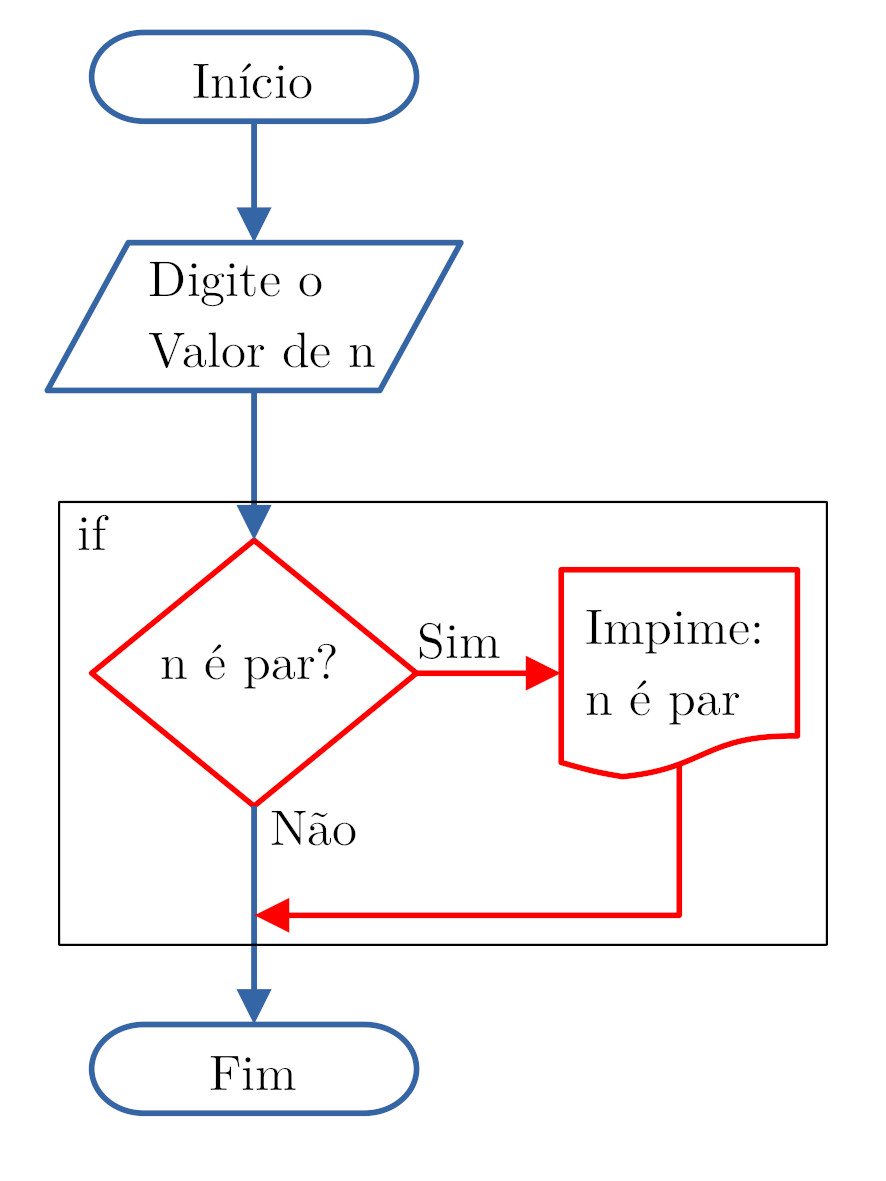
\includegraphics[width=0.5\textwidth]{./cap_progest/dados/fig_fg_ramifica/fig}
  \caption{Fluxograma de uma estrutura de ramificação.}
  \label{cap_progest:fig:fg_ramifica}
\end{figure}
  
\end{ex}

\begin{obs}\normalfont{\hl{(Escopo e indentação.)}}
  Na linguagem {\python}, a \href{https://pt.wikipedia.org/wiki/Indenta\%C3\%A7\%C3\%A3o}{indentação} indica o \emph{escopo}, i.e. o início e fim do bloco de instruções que pertencem a ramificação. No Exemplo \ref{cap_progest_sec_est:ex:ramifica}, o escopo da instrução \lstinline+if+ é apenas a linha 8.
\end{obs}

\subsection{Repetição}

\hl{Instruções de repetição permitem que um mesmo bloco seja processado várias vezes em sequência}. Em {\python}, há duas instruções de repetição disponíveis: \lstinline+for+ e \lstinline+while+. 

\subsubsection{\lstinline+for+}

A instrução \hl{{\lstinline+for+} permite que um bloco seja iterado para cada elemento de uma dada coleção de dados}.

\begin{ex}\label{cap_progest_sec_est:ex:for}
  O seguinte código testa a paridade de cada um dos elementos do conjunto $\{-3, -2, -1, 0, 1, 2, 3\}$.
\begin{lstlisting}
#início

# repetição for
for n in {-3, -2, -1, 0, 1, 2, 3}:
    res = (n%2 == 0)
    print(f'{n} é par? ', res)
    
#término
\end{lstlisting}
  A instrução de repetição \lstinline+for+ (linha 4), aloca em \lstinline+n+ um dos elementos do conjunto. Então, executa em sequência o bloco de comandos das linhas 5 e 6. De forma iterada, \lstinline+n+ recebe um novo elemento do conjunto e o bloco das linhas 5 e 6 é novamente executado. A repetição termina quando todos os elementos do conjunto já tiverem sido iterados. O código segue, então, para a linha 7. Não havendo mais instruções, o programa é encerrado.

\begin{figure}[H]
  \centering
  \includegraphics[width=0.6\textwidth]{./cap_progest/dados/fig_fg_for/fig}
  \caption{Fluxograma de uma estrutura de repetição do tipo \lstinline+for+.}
  \label{cap_progest_sec_est:fig:fg_for}
\end{figure}

Assim como no caso de uma instrução de ramificação, \hl{o escopo do {\lstinline+for+} é definido pela indentação do código}. Neste exemplo, o escopo são as linhas 5 e 6.
\end{ex}

\subsubsection{\lstinline+while+}

A instrução \hl{{\lstinline+while+}, permite a repetição de um bloco enquanto uma dada condição lógica é satisfeita}.

\begin{ex}\label{cap_progest_sec_est:ex:while}
  O seguinte código testa a paridade dos números inteiros compreendidos de $-3$ a $3$.
\begin{lstlisting}
#início

n = -3

# repetição: while
while (n <= 3):
    res = (n%2 == 0)
    print(f'{n} é par?', res)
    n += 1
    
#término
\end{lstlisting}
  A instrução de repetição \lstinline+while+ faz com que o bloco de processamento definido pelas linhas 7-9 seja executado de forma sequencial enquanto o valor de \lstinline+n+ for menor ou igual a 3. No caso dessa condição ser verdadeira, o bloco (linhas 7-9) é executado e, então a condição é novamente verificada. No caso da condição ser falsa, esse bloco não é executado e o código segue para a linha 10. Não havendo mais nenhuma instrução, o programa é encerrado.

  \begin{figure}[H]
    \centering
    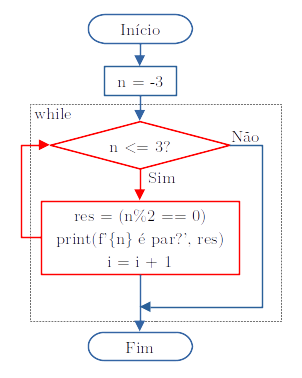
\includegraphics[width=0.6\textwidth]{./cap_progest/dados/fig_fg_while/fig}
    \caption{Fluxograma de uma estrutura de repetição do tipo \lstinline+while+.}
    \label{cap_progest_sec_est:fig:fg_while}
  \end{figure}

  Observamos que, neste exemplo, \hl{o escopo da instrução {\lstinline+while+}} são as linhas 7-9, \hl{determinado indentação do código}.
\end{ex}

\subsection{Exercícios}

\begin{exer}
  Seja a reta de equação
  \begin{equation}
    y = ax + b.
  \end{equation}
  Assumindo $a=2$ e $b=-3$, o seguinte código foi desenvolvido para computar o ponto $x$ de interseção da desta reta com o eixo das abscissas.
\begin{lstlisting}
x = -b/(2*a)
a = 2
b = -3
print(x)
\end{lstlisting}
  Identifique e explique os erros desse código. Então, apresente uma versão corrigida.
\end{exer}
\begin{resp}
\begin{lstlisting}
a = 2
b = -3
x = -b/(2*a)
print(x)
\end{lstlisting}
\end{resp}

\begin{exer}\label{cap_progest_sec_est:exer:ramifica_reta}
  Seja a reta de equação
  \begin{equation}
    y = ax + b.
  \end{equation}
  Faça um fluxograma de um programa em que a(o) usuária(o) entra com os valores de $a$ e $b$. No caso de $a\neq 0$, o programa computa e imprime o ponto $x$ da interseção dessa reta com o eixo das abscissas.
\end{exer}
\begin{resp}
  Dica: consulte o Exemplo \ref{cap_progest_sec_est:ex:ramifica}.
\end{resp}

\begin{exer}
  Implemente o código referente ao fluxograma criado no Exercício \ref{cap_progest_sec_est:exer:ramifica_reta}.
\end{exer}
\begin{resp}
\begin{lstlisting}
a = float(input('Digite o valor de a:\n'))
b = float(input('Digite o valor de b:\n'))
if (a != 0):
    x = -b/(2*a)
    print(f'Ponto de interseção com o eixo x = {x}')
\end{lstlisting}
\end{resp}

\begin{exer}\label{cap_progest_sec_est:exer:for}
  Faça o fluxograma de um programa que usa de um bloco de repetição \lstinline+for+ para percorrer o conjunto
  \begin{equation}
    A = \{-4, -3, -2, -1, 0, 1, 2, 3, 4\}.
  \end{equation}
  A cada iteração, o programa imprime \lstinline+True+ ou \lstinline+False+ conforme o elemento seja ímpar ou não.
\end{exer}
\begin{resp}
  Dica: consulte o Exemplo \ref{cap_progest_sec_est:ex:for}.
\end{resp}

\begin{exer}
  Implemente o código referente ao fluxograma criado no Exercício \ref{cap_progest_sec_est:exer:for}.
\end{exer}
\begin{resp}
\begin{lstlisting}
A = {-4, -3, -2, -1, \
     0, 1, 2, 3, 4}
for x in A:
    res = (x % 2 != 0)
    print(f'{x} é ímpar? {res}')
\end{lstlisting}
\end{resp}

\begin{exer}\label{cap_progest_sec_est:exer:while}
  Faça um fluxograma análogo ao do Exercício \ref{cap_progest_sec_est:exer:for} que use a instrução de repetição \lstinline+while+ no lugar de \lstinline+for+.
\end{exer}
\begin{resp}
  Dica: consulte o Exemplo \ref{cap_progest_sec_est:ex:while}.
\end{resp}

\begin{exer}
  Implemente um código referente ao fluxograma criado no Exercício \ref{cap_progest_sec_est:exer:while}.
\end{exer}
\begin{resp}
\begin{lstlisting}
A = {-4, -3, -2, -1, \
     0, 1, 2, 3, 4}
n = -4
while (n <= 4):
    res = (n % 2 != 0)
    print(f'{n} é ímpar? {res}')
    n += 1
\end{lstlisting}
\end{resp}

\section{Instruções de Ramificação}\label{cap_progest_sec_ramifica}

[[tag:construcao]]

\subsection{Exercícios}

[[tag:construcao]]